\section{Introduction}

The problem of string matching has been studied extensively
due to its wide range of applications from Internet searches to computational biology. 
String matching can be defined as follows. Given a text $T=t_1 t_2\cdots
t_n$ and a pattern $P=p_1p_2\cdots p_m$, with letters from an alphabet $\Sigma$,
find all the occurrences of the pattern in the text.
This problem can be solved in $O(n+m)$ time by using well known algorithms
(e.g., KMP \cite{KMP77}). A variation of this problem is to search for
multiple patterns at the same time. An algorithm for this version is given in 
\cite{AC75}. The problem has been generalized to use trees instead of sequences
or to use sets of characters instead of single characters (see \cite{CH99}). 


A more general formulation allows ``don't care'' or ``wild card''
characters in the text and the pattern. A wild card matches any character. An 
algorithm for pattern matching with wild cards is given in \cite{FP74} and has a
runtime of $O(n \log |\Sigma| \log m)$.  The algorithm maps each character in
$\Sigma$ to a binary code of length $\log |\Sigma|$. Then, a constant number of
convolution operations are used to check for mismatches between the
pattern and any position in the text. For the same problem, a randomized algorithm
that runs in $O(n \log n)$ time with high probability is given
in \cite{IND98}. A slightly faster randomized $O(n \log m)$ algorithm is given in
\cite{Kal02}. A simple deterministic $O(n \log m)$ time algorithm based on
convolutions is given in \cite{CC07}.

A more challenging formulation of the problem is pattern matching with
mismatches.
This formulation appears in two versions: a) for every alignment of the
pattern in the text, find the distance between the pattern and the text,
or b) identify only those alignments where the distance between the pattern and the text is less than a given
threshold. The distance metric can be the Hamming distance, edit
distance, $L_1$ metric, and so on. 
A survey of string matching with mismatches is given in \cite{Nav01}.
A description of practical on-line string searching algorithms can be
found in \cite{NR02}.

The algorithms in this chapter are using
the Hamming distance. The Hamming distance between two strings $A$ and $B$, of equal
length, is defined as the number of positions where the two strings differ and is denoted
by $Hd(A,B)$. We are interested in the following two problems, with and without
wild cards.
 

{\bf 1. Pattern matching with mismatches:} Given a text $T=t_1t_2\ldots
t_n$, and a pattern $P=p_1p_2\ldots p_m$, output $Hd(P, t_i t_{i+1}\ldots
t_{i+m-1})$, for every $i,~1\leq i\leq n-m+1$.

{\bf 2. Pattern matching with $k$ mismatches (or the $k$-mismatches problem):}
Take the same input as above, plus an integer $k$. Output all $i$, $1\leq i\leq
n-m+1$, for which $Hd(P, t_i t_{i+1},\ldots t_{i+m-1}) \leq k$.


\subsection{Pattern Matching with Mismatches}

For pattern matching with mismatches, a naive algorithm
computes the Hamming distance for every alignment of the pattern in the
text, in time $O(nm)$. A faster algorithm, in the absence of wild cards, is
Abrahamson's algorithm \cite{ABR87} that runs in $O(n \sqrt{m \log m})$
time.
Abrahamson's algorithm can be extended to solve pattern matching
with mismatches {\em and} wild cards, as we prove in section \ref{sec_glogm}.
The new algorithm runs in $O(n \sqrt{g \log m})$ time, where $g$ is the number of non-wild card positions in the pattern. This gives a simpler and
faster alternative to an algorithm proposed in \cite{ALP04}.

In the literature, we also find algorithms that approximate the number of
mismatches for every alignment. For example, an approximate algorithm for
pattern matching with mismatches, in the absence of wild cards, that runs in $O(r n \log
m)$ time, where $r$ is the number of iterations of the algorithm, is
given in \cite{ACD01}. Every distance reported has a variance bounded by
$(m-c_i)/{r^2}$ where $c_i$ is the exact number of matches for alignment $i$.

Furthermore, a randomized algorithm that approximates the Hamming distance
for every alignment within an $\epsilon$ factor and runs in $O(n
\log^cm/\epsilon^2)$ time, in the absence of wild cards, is given in \cite{KAR93}.
Here $c$ is a small constant. We extend this algorithm to
pattern matching with mismatches {\em and} wild cards, in
section \ref{sec_approx_count_rand}.
The new algorithm
approximates the Hamming distance for every alignment within an $\epsilon$ factor in time
$O(n\log^2m/\epsilon^2)$ with high probability.

Recent work has also addressed the online
version of pattern matching, where the text is received in a
streaming model, one character at a time, and it cannot be stored in its
entirety (see e.g., \cite{CKP08}, \cite{PP09}, \cite{PL07}).
Another version of this problem matches the pattern against multiple input
streams (see e.g., \cite{CEP+07}). Another interesting problem is to sample a
representative set of mismatches for every alignment (see e.g., \cite{CEP+12}).

\subsection{Pattern Matching with $k$ Mismatches}

For the $k$-mismatches problem, without wild cards, two algorithms that
run in $O(nk)$ time are presented in \cite{LV85} and \cite{GG86}. A faster
algorithm, that runs in $O(n\sqrt{k \log k})$ time, is given in
\cite{ALP04}. This algorithm combines the two
main techniques known in the literature for pattern matching with mismatches: filtering and convolutions. 
We give a significantly simpler algorithm in section \ref{sec_nsqrtk}, having
the same worst case run time. The new algorithm will never perform more
operations than the one in \cite{ALP04} during marking and convolution. 
 
An intermediate problem is to check if the
Hamming distance is less or equal to $k$ for a subset of the aligned positions.
This problem can be solved with the Kangaroo method proposed in \cite{GG86} at a
cost of $O(k)$ time per alignment, using $O(n+m)$ additional memory. We show how to achieve the same
run time per alignment using only $O(m)$ additional memory, in section
\ref{sec_k_mism_det}.

Further, we look at the version of $k$-mismatches where wild cards are allowed
in the text and the pattern. For this problem, two randomized algorithms are
presented in \cite{CEP+07}. The first one runs in $O(nk\log n\log m)$  time and
the second one in $O\left (n\log m(k+\log n\log\log n)\right )$ time.
Both are Monte Carlo algorithms, i.e., they output the correct
answer with high probability. The same paper also gives a deterministic
algorithm with a run time of $O(nk^2\log^3m)$. Also, a deterministic $O(nk
\log^2 m(\log^2 k + \log \log m))$ time algorithm is given in \cite{CEPR09}. We present a
Las Vegas algorithm (that always outputs the correct answer), in section
\ref{sec_las_vegas}, which runs in time $O(nk\log^2 m+n\log^2m\log n+n\log
m\log n\log\log n)$ with high probability. Deterministically, pattern matching
with $k$ mismatches and wild cards can be solved in time $O(nk^2\log^2m)$ as shown in
\cite{Clif10}.

If we allow for wild cards in the pattern but not the text, an 
$O(nm^{1/3}k^{1/3}log^{2/3}m)$ time algorithm is given in \cite{CP10}.
We improve this runtime as follows.  Given a pattern $P$, with wild cards, a
maximal length substring of $P$ that has no wild cards is called an ``island''.
We denote the number of islands in $P$ as $q$. In chapter 
\ref{sec_nsqrtk_wild} we give two algorithms for pattern matching with $k$
mismatches where there are wild cards in the pattern.
The first one runs in $O(n\sqrt{(q+k)\log m})$ time. 
The second one runs in time $O(n\sqrt[3]{qk\log^2 m} +
n\sqrt{k\log m})$ where $q$ is the number of islands in $P$. By combining the
two, we show that pattern matching with $k$ mismatches and wild cards in the
pattern can be solved in $O(n\sqrt{k\log m}+n\min\{\sqrt[3]{qk\log^2 m},\sqrt{q\log m}\})$ time.
If the number of islands is $O(k)$ our runtime becomes $O(n\sqrt{k \log m})$,
which essentially matches the best known runtime for pattern matching with $k$
mismatches without wild cards ($O(n\sqrt{k\log k})$). 
 If $q=o(m)$, our algorithm outperforms the
$O(n\sqrt[3]{mk\log^2m})$ run time of \cite{CP07}.  
Therefore, our algorithm is a step
towards bridging the gap between the versions with and without wild cards
cares for pattern matching with $k$ mismatches. 
%ADD
In other words, with the
previous algorithm, even with a few wild cards in the pattern, the
runtime could be much larger than the runtime if there were no wild cards.
In the new algorithm, if the number of wild cards is relatively small
then the runtime is the same as in the version without wild cards.
%%% 



\subsection{Our Results}

The contributions of this chapter can be summarized as follows.

{\bf For pattern matching with mismatches:}
\begin{itemize}
\item An algorithm  for pattern matching with mismatches
and wild cards that runs in $O(n \sqrt{g \log m})$ time, where $g$ is the
number of non-wild card positions in the pattern. See section \ref{sec_glogm}.

\item A randomized algorithm that approximates the Hamming distance for every
alignment, when wild cards are present, within an $\epsilon$ factor in time
$O(n\log^2m/\epsilon^2)$ with high probability. See section
\ref{sec_approx_count_rand}.
\end{itemize}

{\bf For pattern matching with $k$ mismatches:}
\begin{itemize}
\item An algorithm that tests if the Hamming distance is less than $k$
for a subset of the alignments, without wild cards, at a cost of $O(k)$ time per
alignment, using only $O(m)$ additional memory. This achieves the same
runtime per alignment as the Kangaroo method, but with less memory. See section
\ref{sec_k_mism_det}.

\item An algorithm for pattern matching
with $k$ mismatches, without wild cards, that runs in $O(n\sqrt{k \log k})$
time. This algorithm is simpler and has a better expected run time than the one
in \cite{ALP04}. See section \ref{sec_nsqrtk}.

\item An algorithm for pattern matching
with $k$ mismatches with wild cards in the pattern, that runs
in $O(n\sqrt{k\log m}+n\min\{\sqrt[3]{qk\log^2 m},\sqrt{q\log m}\})$ time,
where $q$ is the number of non-wild card islands in the pattern.  If $q=o(m)$,
our algorithm outperforms the $O(n\sqrt[3]{mk\log^2m})$ run time of \cite{CP07}.
See section \ref{sec_nsqrtk_wild}.


\item A Las Vegas algorithm for the
$k$-mismatches problem with wild cards that runs in
time $O(nk\log^2 m+n\log^2m\log n+n\log m\log n\log\log n)$ with high
probability. See section \ref{sec_las_vegas}.
\end{itemize}

These algorithms are also included in our papers \cite{NRKM15} and
\cite{NRKM16}.
The rest of the chapter is organized as follows. First we introduce some notations
and definitions. 
Then we describe the exact, deterministic algorithms for pattern matching with
mismatches and for $k$-mismatches. Then we present the randomized and
approximate algorithms: first the algorithm for approximate counting of
mismatches in the presence of wild cards, then the Las Vegas algorithm for
$k$-mismatches with wild cards. Finally, we present an empirical run time
comparison of the deterministic algorithms, and conclusions.

\section{Materials and Methods}

In terms of notation, $T_{i..j}$ is the substring of $T$ between $i$ and $j$
and $T_i$ stands for $T_{i..i+m-1}$. Furthermore, the value at
position $i$ in array $X$ is denoted by $X[i]$. 

%%%%%%%%%%%%%%%%%%

\subsection{Background}
In this section we review a number of well known
techniques used in the literature for pattern pattern matching with $k$ mismatches (e.g., see
\cite{ALP04}), namely: convolution, marking, filtering and the Kangaroo method.




 

\subsubsection{Convolution}
Given two arrays $T=t_1t_2\ldots t_n$ and $P=p_1p_2\ldots
p_m$ (with $m\leq n$), the convolution of $T$ and $P$ is a sequence
$C=c_1,c_2,\ldots,c_{n-m+1}$ where $c_i=\sum_{j=1}^mt_{i+j-1}p_j$, for $1\leq
i\leq (n-m+1)$. 

The convolution can be applied to pattern matching with mismatches, as follows.
Given a string $S$ and a character $\alpha$ define string $S^{\alpha}$
as $S^\alpha[i]=1$ if $S[i]=\alpha$ and $0$ otherwise.
Let $C^\alpha=convolution(T^\alpha, P^\alpha)$. Then $C^\alpha[i]$ gives the
number of matches between $P$ and $T_i$
where the matching character is $\alpha$. Therefore, one convolution gives us
the number of matches contributed by a single character to each of the
alignments. Then $\sum_{\alpha \in \Sigma}C^{\alpha}[i]$ is the total number of
matches between $P$ and $T_i$.

One convolution can be computed in
$O(n\log m)$ time by using the Fast Fourier Transform. 
If the convolutions are applied on binary inputs, as is often the case in
pattern matching applications, some speedup techniques are presented in \cite{FG09}.

\subsubsection{Marking}\label{sec_marking} 

Marking is an algorithm that counts the number of matches of
every alignment.
Specifically, the algorithm scans the text one character at a time
and ``marks'' all the alignments that would produce a match between the current
character in the text and the corresponding character in the pattern. 

The marking algorithm is generally used only on a subset of the pattern. That
is, given a set $A$ of positions in $P$ the marking algorithm counts matches
between the text and the subset of $P$ given by $A$. The pseudocode of the
marking algorithm is given in Algorithm \ref{alg_counting}.

\begin{algorithm}
\SetKwInOut{Input}{input}\SetKwInOut{Output}{output}
\caption{Mark$(T, P, A)$}\label{alg_counting} 
\Input{Text $T$, pattern $P$ and a set $A$ of positions in $P$} 
\Output{An array $M$ where $M[i]$ gives the number of matches between $T_i$
and $P$, on the subset of positions of $P$ given by $A$}
\lFor {$i\leftarrow 1$ \KwTo $n$}{$M[i]=0$}
\For {$i\leftarrow 1$ \KwTo $n$}{
  \For{$j \in A$ s.t. $P[j] = T[i]$}{
    \lIf{$i-j+1 > 0$}{
      $M[i-j+1]${\bf $++$}
    }
  }
}
\Return $M$\;
\end{algorithm}

\subsubsection{Filtering}
The marking algorithm in the previous section is generally followed by a
filtering method. Filtering is based on the following principle. If we restrict
our pattern to only $2k$ positions, any alignment that has no more than
$k$ mismatches, must have at least $k$ matches among the $2k$ positions.
To count matches among the $2k$ positions selected, for every alignment, we use
the marking algorithm. If the total number of marks generated is $B$ then there
can be no more than $B/k$ positions that have at least $k$ marks (i.e.,
matches). The alignments that have at least
$k$ marks are further inspected using the Kangaroo method.

\subsubsection{The Kangaroo method}\label{sec_kangaroo} 

The Kangaroo method allows us to check if the number of mismatches for a
particular alignment is no more than $k$, in $O(k)$ time. The Kangaroo method
constructs a generalized suffix tree of $T\#P$ where $\#$ means concatenation.
This suffix tree can be enhanced to answer Lowest Common Ancestor
(LCA) queries in $O(1)$ time \cite{AH+76}. LCA queries give us the longest
common prefix between any portion of the text and any portion of the pattern,
essentially telling us where the first mismatch appears. 
Specifically, to count mismatches between
$P$ and $T_i$, first perform an LCA query to find the position of the
first mismatch between $P$ and $T_i$. Let this position be $j$. Then,
perform another LCA to find the first mismatch between $P_{j+1..m}$ and
$T_{i+j+1.. i+m-1}$, which gives the second mismatch of alignment $i$.
Continue to ``jump'' from one mismatch to the next, until the end
of the pattern is reached or we have found more than $k$ mismatches.
Therefore, after $O(k)$ LCA queries we will either find all the mismatches or
determine that there are more than $k$ of them. 
The Kangaroo pseudocode is given in Algorithm \ref{alg_kangaroo}.

\begin{algorithm}
\SetKw{LCA}{LCA}
\SetKw{True}{true}
\SetKw{False}{false}
\SetKwInOut{Input}{input}\SetKwInOut{Output}{output}
\caption{Kangaroo$(P, T_i, k)$}\label{alg_kangaroo}
\Input{A pattern $P$, an alignment $T_i$ and an integer $k$}
\Output{\True if the pattern matches the alignment with no more than $k$
mismatches, \False otherwise}
$j=0$\;
$d=0$\;
\While{$d \leq k$} {
  $j = j + \LCA(T_{i+j}, P_j)+1$\;
  \If {$j > m$} {
     \Return{\True}\;
  }
  $d=d+1;$
}  
\Return{\False}\;
\end{algorithm}

\subsubsection{Probability Bounds}
 
In the context of randomized algorithms, by
high probability we mean a probability greater or equal to $(1-n^{-\epsilon})$ 
where $n$ is the input size and $\epsilon$ is a probability parameter usually
assumed to be a constant greater than $0$. The run time of a Las Vegas algorithm
is said to be $\widetilde O(f(n))$ if the run time is no more than $c\epsilon f(n)$
with probability greater or equal to $(1-n^{-\epsilon})$ for all $n\geq n_0$,
where $c$ and $n_0$ are some constants, and for any constant $\epsilon\geq 1$.


In the analysis of our algorithms, we will employ the following Chernoff bounds.


\noindent{\bf Chernoff Bounds} \cite{Che52}.
These bounds can be used to closely
approximate the tail ends of a binomial distribution.

A Bernoulli trial has two outcomes namely {\em success} and {\em failure},
the probability of success being $p$. A binomial distribution with
parameters $n$ and $p$, denoted as $B(n,p)$, is the number of successes
in $n$ independent Bernoulli trials.

Let $X$ be a binomial random variable whose distribution is
$B(n,p)$. If $m$ is any integer $>np$, then the following are true:
\begin{equation}\label{eq_chernoff1}
Prob.[X>m]~\leq~\left (\frac{np}{m}\right )^m~e^{m-np};
\end{equation}

\begin{equation}\label{eq_chernoff2}
Prob.[X>(1+\delta)np]~\leq~e^{-\delta^2np/3};~{\rm and}
\end{equation}

\begin{equation}\label{eq_chernoff3}
Prob.[X<(1-\delta)np]~\leq~e^{-\delta^2np/2}
\end{equation}
 for any
$0<\delta<1$.

\subsection{Exact Algorithms for Pattern Matching with Mismatches}


For pattern matching with mismatches, without wild cards,
the following $O(n\sqrt{m \log m})$ time algorithm was given by Abrahamson
\cite{ABR87}.
Let $A$ be a set of the most frequent characters
in the pattern. 1) Using convolutions, count how many matches each character in $A$ contributes to
every alignment. 2) Using marking, count how many matches each character
in $\Sigma - A$ contributes to every alignment. 3) Add the two
numbers to find for every alignment, the number of matches between the pattern
and the text. The convolutions take $O(|A| n \log m)$ time. A
character in $\Sigma - A$ cannot appear more than $m/|A|$ times in the pattern,
otherwise, each character in $A$ has a frequency greater than
$m/|A|$, which is not possible. Thus, the run time for marking is $O(n m / |A|)$.
If we equate the two run times we find the optimal $|A| = \sqrt{m / \log m}$ which gives a
total run time of $O(n \sqrt{m \log m})$.


\noindent{\bf An Example.} Consider the case of $T=2~3~1~1~4~1~2~3~4~4~2~1~1~3~2$ and $P=1~2~3~4$. Since each character in the pattern occurs an equal number of times, we can pick $A$ arbitrarily. Let $A=\{1,2\}$. In step 1, convolution is used to count the number of matches contributed by each character in $A$. We obtain an array $M_1[1:12]$ such that $M_1[i]$ is the number of matches contributed by characters in $A$ to the alignment of $P$ with $T_i$, for $1\leq i\leq 12$. In this example, $M_1=[0,0,1,1,0,2,0,0,0,1,0,1]$. In step 2 we compute, using marking, the number of matches contributed by the characters $3$ and $4$ to each alignment between $T$ and $P$. We get another array $M_2[1:12]$ such that $M_2[i]$ is the number of matches contributed by $3$ and $4$ to the alignment between $T_i$ and $P$, for $1\leq i\leq 12$. Specific to this example, $M_2=[0,1,0,0,0,2,1,0,0,0,0,1]$. In step 3, we add $M_1$ and $M_2$ to get the number of matches between $T_i$ and $P$, for $1\leq i\leq 12$. In this example, this sum yields: $[0,1,1,1,0,4,1,0,0,1,0,2]$.


\subsubsection{Pattern matching with mismatches and wild cards in $O(n\sqrt{g
\log{g}})$}
\label{sec_glogm}
For pattern matching with mismatches and wild cards, 
a fairly complex algorithm is given in \cite{ALP04}. The run time of this
algorithm is $O(n \sqrt{g} \log m)$ where $g$ is the number of non-wild card
positions in the pattern. The problem can also be solved through a simple modification of 
Abrahamson's algorithm, in time $O(n\sqrt{m \log m})$, as pointed out in 
\cite{CEP+07}. We now prove the following result:

\begin{theorem}
\label{thm_glogm}
 Pattern matching with mismatches and wild cards can be solved
in $O(n\sqrt{g \log m})$ time, where $g$ is the number of non-wild card
positions in the pattern.
\end{theorem}

\begin{proof}
 Ignoring the wild cards for now, let $A$ be the set of
the most frequent characters in the pattern. As above, count matches contributed
by characters in $A$ and $\Sigma-A$ using convolution and marking, respectively.
By a similar reasoning as above, the characters used in the marking phase will not 
appear more than $g / |A|$ times in the pattern. If we equate the run times for the two 
phases we obtain $O(n \sqrt {g \log m})$ time. We are now left to count how many matches are
contributed by the wild cards. For a string $S$ and a character $\alpha$, define $S^{\neg \alpha}$ as
$S^{\neg \alpha}[i] = 1-S^\alpha[i]$. Let
$w$ be the wild card character. Compute $C = convolution(T^{\neg w}, P^{\neg w})$. Then,
for every alignment $i$, the number of positions that have a wild card either in the
text or the pattern or both, is $m-C[i]$. Add $m-C[i]$ to the previously computed counts and output. 
The total run time is $O(n \sqrt{g \log m})$.
\end{proof}

\subsection{Exact Algorithms for Pattern Matching with $k$ Mismatches}
\label{sec_k_mism_det}

For the $k$-mismatches problem, without wild cards, an $O(k(m\log m+n))$ time
algorithm that requires $O(k(m+n))$ additional space is presented in \cite{LV85}. Another algorithm, that takes
  $O(m\log m + kn)$ time and uses only $O(m)$ additional space is presented
in \cite{GG86}. \commentOut{In the latter, a suffix tree of the pattern is built and enhanced to
support lowest common ancestor queries in $O(1)$ time.} We define the following
problem which is of interest in the discussion.

\subsubsection{The Subset $k$-mismatches problem}
\begin{problem}
{\bf Subset $k$-mismatches:} Given a text $T$ of length $n$, a pattern $P$ of
length $m$, a set of positions $S=\{i|1 \leq i \leq n-m+1\}$ and an integer $k$, output the
positions $i \in S$ for which $Hd(P, T_i) \leq k$.
\end{problem}

The Subset $k$-mismatches problem becomes the regular $k$-mismatches
problem if $|S|=n-m+1$. Thus, it can be solved by the $O(nk)$ algorithms mentioned
above. However, if $|S| << n$ then the
$O(nk)$ algorithms are too costly.
A better alternative is to use the Kangaroo method proposed in \cite{ALP04} and
described in section \ref{sec_kangaroo}. The Kangaroo method can verify if
$Hd(P, T_i)\leq k$ in $O(k)$ time for any $i$. The
Kangaroo method can process $|S|$ positions in $O(n+m+|S|k)$ time and it
uses $O(n+m)$ additional memory for the LCA enhanced suffix tree.
The memory requirement can be improved as follows:

\begin{theorem}
{\bf Subset $k$-mismatches} can be solved in $O(n+m+|S|k)$ time using only
$O(m)$ additional memory.
\end{theorem}


\begin{proof}
The algorithm  is the following. Build an LCA-enhanced suffix tree
 of the pattern. Scan the text from left to right. 1) Find the longest unscanned region
of the text that can be found somewhere in the pattern, say starting at
position $i$ of the pattern. Call this region of the text $R$. Therefore, $R$ is
identical to $P_{i..i+|R|-1}$. 2) For every alignment in $S$ that overlaps $R$, count
the number of mismatches between $R$ and the alignment, within the overlap
region.
To do this, consider an alignment in $S$ which overlaps $R$ such that the
beginning of $R$ aligns with the $j$-th character in the pattern. We want to count the number of mismatches between R and $P_{j..j+|R|-1}$. However, since $R$ is identical to
$P_{i..i+|R|-1}$, we can simply compare $P_{i..i+|R|-1}$ and
$P_{j..j+|R|-1}$. This comparison can be done efficiently by jumping from one
mismatch to the next, like in the Kangaroo method. Repeat from step 1 until the
entire text has been scanned.
Every time we process an alignment, in step 2, we either discover at least one additional
mismatch or we reach the end of the alignment.
This is true because, otherwise, the alignment
would match the text for more than $|R|$ characters, which is not possible, from
the way we defined $R$. Every alignment for which we have found more than $k$
mismatches is excluded from further consideration to ensure
$O(k)$ time per alignment. It takes $O(m)$ time to build the LCA enhanced suffix tree of the pattern and
$O(n)$ additional time to scan the text from left to right. Thus, the total run time is
$O(n+m+|S|k)$ with $O(m)$ additional memory. The pseudocode is given in
Algorithm \ref{alg_subsetk}.
\end{proof}

{\LinesNumberedHidden
\begin{algorithm}
\SetKw{And}{and}
\SetKwFunction{updateMism}{countMismatches}
\SetKwFunction{lcp}{lcp}
\SetKwInOut{Input}{input}\SetKwInOut{Output}{output}
\caption{Subset $k$-mismatches($S, T, P, k$)}\label{alg_subsetk} 
\Input{$S$ - set of positions in the text; $T_{1..n}$ - text; $P_{1..m}$
-pattern; k - max number of mismatches\;} 
\Output{$M$ - the positions in $S$ for which the pattern matches the text with
at most $k$ mismatches\;} 
\Begin{
Assume we have a suffix tree/array of the pattern\;
\lFor {$a \in S$}{$M[a]=0$}
$i=1$ \;
\While{$i \leq n$} {
Find the largest $l$ such that $T_{i..i+l-1}$ describes a path in the suffix
tree\; 
This means that $T_{i..i+l-1} = P_{j..j+l-1}$ for some $j$\;
\For{$a \in S$ {\bf where} $a \leq i < a + m$} { 
$M[a] =$ \updateMism$(M[a],
i-a+1, j, l)$ \;
\lIf{$t_{i+l}\neq p_{j+l}$}{$M[a]=M[a]+1$}
\lIf {$M[a] > k$} {$S = S - \{a\}$}
}
$i = i + l + 1$ \;
}
\Return{$\{a \in S | M[a]\leq k\}$}
}
\SetKwProg{myproc}{function}{}{}
\myproc{\updateMism{$c, s_1, s_2, l$}}{
\Input{$c$ - current number of mismatches; $s_1, s_2$ - starting positions of
two suffixes of the pattern; $l$ - a maximum length\;}
\Output{compare the two suffixes on their first $l$ positions and add to $c$
the number of mismatches found; if $c$ exceeds $k$, return $k+1$,
otherwise return the updated $c$ \;} 
\Begin{ \While{$l > 0$  \And $c \leq k$}{
  $d = \lcp(s_1,s_2)$; // longest common prefix\\
  \lIf {$d \geq l$}{\Return {$c$}} 
  $c = c + 1$\;
  $d = d + 1$\;
  $s_1 = s_1 + d$\;
  $s_2 = s_2 + d$\; 
  $l = l - d$\;
}
}
\Return{$c$}
}
\end{algorithm}
}


\subsubsection{An $O(n\sqrt{k \log k})$ Time Algorithm for $k$-Mismatches
without Wild Cards}
\label{sec_nsqrtk}
 
For the $k$-mismatches problem, without wild cards, a fairly complex 
$O(n \sqrt{k \log k})$ time algorithm  is given in \cite{ALP04}. 
The algorithm classifies the inputs into several cases. For each case
it applies a combination of marking followed by a filtering step, the Kangaroo
 method, or convolutions. The goal is to not exceed $O(n \sqrt{k \log k})$ time 
 in any of the cases.
We now present an algorithm with only two cases which has the same worst case run time.
The new algorithm can be thought of as a generalization of the algorithm in \cite{ALP04} 
as we will discuss later.
This generalization not only greatly simplifies the algorithm but it also
reduces the expected run time. This happens because we use information about the frequency of the
characters in the text and try to minimize the work done by convolutions and marking.

We will now give the intuition for this algorithm. For any
character $\alpha \in \Sigma$, let $f_\alpha$ be its frequency in the pattern,
and $F_\alpha$ be its frequency in the text. Note that in the marking algorithm,
a specific character $\alpha$ will contribute to the runtime a cost of
$F_{\alpha} \times f_{\alpha}$. On the other hand, in the case of convolution, a
character $\alpha$ costs us one convolution, regardless of how frequent $\alpha$
is in the text or the pattern. Therefore, we want to use infrequent
characters for marking and frequent characters for convolution. The balancing of
the two will give us the desired runtime.

A position $j$ in
the pattern where $p_j = \alpha$ is called an {\em instance} of $\alpha$. 
Consider every instance of character $\alpha$ as an object of size
$1$ and cost $F_\alpha$. We want to fill a knapsack of size $2k$ at a minimum
cost and without exceeding a given budget $B$. The $2k$
instances will allow us to filter some of the alignments with more
than $k$ mismatches, as it will become clear later. This
problem can be optimally solved by a greedy approach where we include in the knapsack all the instances of the least expensive character, then all the instances of the second least expensive character and so on, until we have $2k$ items or we have exceeded $B$. The last
character considered may have only a subset of its instances included, but for
ease of explanation assume that there are no such characters.

{\bf Note:} Even though the above is described as a Knapsack problem, the
particular formulation can be optimally solved in linear time. This formulation should not be
confused with other formulations of the Knapsack problem that are NP-Complete.

Case 1) Assume we can fill the knapsack at a cost $C \leq B$. We apply the
marking algorithm for the characters whose instances are included in the
knapsack. It is easy to see that the marking takes time $O(C)$ and creates $C$
marks. For alignment $i$, if the pattern and the text match for all the $2k$
positions in the knapsack, we will obtain exactly $2k$ marks at position $i$. 
Conversely, any position which has less than $k$ marks must have more
than $k$ mismatches, so we can filter it out. Therefore, there will be at
most $C/k$ positions with $k$ marks or more. For such positions we run Subset
$k$-mismatches to confirm which of them have less than $k$ mismatches.
The total runtime of the algorithm in this case is $O(C)$.

Case 2) If we cannot fill the knapsack within the given budget $B$ we do the
following: for the characters we could fit in the knapsack, we use the marking
algorithm to count the number of matches they contribute to each alignment. For
characters not in the knapsack, we use convolutions to count the number of
matches they contribute to each alignment. We add the two counts and get the
exact number of matches for every alignment. 

Note that at
least one of the instances in the knapsack has a cost larger than $B/(2k)$ (if
all the instances in the knapsack had a cost less or equal to $B/(2k)$ then we would
have at least $2k$ instances in the knapsack). Also note that all the
instances not in the knapsack have a cost at least as high as any instance in
the knapsack, because we greedily fill the knapsack starting with the least
costly instances. This means that every character not in the knapsack appears
in the text at least $B/(2k)$ times. This means that the number of characters
not in the knapsack does not exceed $n/(B/(2k))$. Therefore the total cost of
convolutions is $O(nk/B\log m)$. Since the cost of marking was $O(B)$ we can see
that the best value of $B$ is the one that equalizes the two costs. This gives
$B=O(n\sqrt{k\log m})$. Therefore, the algorithm takes $O(n\sqrt{k\log m})$
time. If $k < m^{1/3}$  we can employ a different algorithm
that solves the problem in linear time, as in \cite{ALP04}. For larger $k$,
$O(\log m) = O(\log k)$ so the run time becomes $O(n \sqrt{k \log k})$. We call this algorithm
{Knapsack $k$-mismatches}. The pseudocode is given in algorithm
\ref{alg_knapsack}. The following theorem results.


\begin{theorem}
{\bf Knapsack $k$-mismatches} has worst case run time $O(n \sqrt{k \log
k})$.$\square$
\end{theorem}

{\LinesNumberedHidden
\begin{algorithm}
\SetKw{And}{and}
\SetKwFunction{Mark}{Mark}
\SetKwFunction{convolution}{convolution}
\SetKwFunction{subsetk}{Subset $k$-mismatches}
\SetKwInOut{Input}{input}\SetKwInOut{Output}{output}
\caption{Knapsack $k$-mismatches($T, P, k$)}\label{alg_knapsack}
\Input{$T_{1..n}$ - text; $P_{1..m}$ -pattern; k - max number of mismatches\;} 
\Output{$S$ - set of positions in the text where the pattern matches with at
most $k$ mismatches\;} 
\Begin{
Compute $F_i$ and $f_i$ for every $i \in \Sigma$ \;
Sort $\Sigma$ with respect to $F_i$ \;
$s = 0$\;
$c = 0$\;
$i = 1$\;
$B = n \sqrt{k \log k}$ \;
\While{$s < 2k$ \And $c < B$} {
  $t = \min(f_i, 2k - s)$ \;
  $s = s + t$ \;
  $c = c + t \times F_i$ \;
  $i = i + 1$ \;
}
$\Gamma = \Sigma[1..i]$ \;
$M = \Mark(T, n, \Gamma)$; // $M$ counts matches\\
\eIf {$s = 2k$} {
  $S = \{i | M[i] \geq k\}$  \;
  \Return \subsetk($S, T, P, k$)\;
}{
  \For{$\alpha \in \Sigma - \Gamma$} {
    $C = \convolution(T^{\alpha}, P^{\alpha})$ \;
    \For {$i \leftarrow 1$ \KwTo $n$} {
      $M[i] = M[i] + C[i]$ \;
    }
  }
  $S = \{i | M[i] \geq m-k\}$\;    
  \Return{$S$}\;
}
}
\end{algorithm}
}

We can think of the algorithm in \cite{ALP04} as a special case of our
algorithm where, instead of trying to minimize the cost of the $2k$ items in the
knapsack, we just try to find $2k$ items for which the cost is less than
$O(n\sqrt{k \log m})$. As a result, it is easy to verify the following:
\begin{theorem}\label{knapsack_less}
{\bf Knapsack $k$-mismatches} spends at most as much time as
the algorithm in \cite{ALP04} to do convolutions and marking.
\end{theorem}

\begin{proof}
{\bf Observation:} In all the cases presented below,
Knapsack $k$-mismatches can have a run time as low as $O(n)$, for example if
there exists one character $\alpha$ with $f_\alpha = O(k)$ and $F_\alpha = O(n/k)$.

{\bf Case 1:} $|\Sigma| \geq 2k$. The algorithm in \cite{ALP04} chooses $2k$
instances of distinct characters to perform marking. Therefore, for every
position of the text at most one mark is created. If the number of
marks is $M$, then the cost of the marking phase is $O(n + M)$.
The number of remaining positions after filtering is no more than $M/k$ and thus the algorithm takes
$O(n+M)$ time.
Our algorithm puts in the knapsack 2k instances, of not necessarily different
characters, such that the number of marks $B$ is minimized! Therefore $B \leq M$
and the total runtime is $O(n+B)$.

{\bf Case 2:} $|\Sigma| < 2\sqrt{k}$. The algorithm in \cite{ALP04} performs
one convolution per character to count the total number of matches for every
alignment, for a run time of $\Omega(|\Sigma|n\log m)$. In the worst case, 
Knapsack $k$-mismatches cannot fill the knapsack at a cost $B < |\Sigma|n\log
m$ so it defaults to the same run time. However, in the best case, the
knapsack can be filled at a cost $B$ as low as $O(n)$ depending on the
frequency of the characters in the pattern and the text. In this case the
runtime will be $O(n)$.

{\bf Case 3:} $2\sqrt{k} \leq |\Sigma| \leq 2k$. A symbol that appears in the
pattern at least $2\sqrt{k}$ times is called frequent.

{\bf Case 3.1:} There are at least $\sqrt{k}$ frequent symbols. The algorithm in
\cite{ALP04} chooses $2\sqrt{k}$ instances of $\sqrt{k}$ frequent symbols to do
marking and filtering at a cost $M \leq 2n\sqrt{k}$. Since Knapsack
$k$-mismatches will minimize the marking time $B$ we have
$B \leq M$ so the run time is the same as for \cite{ALP04} only in the worst
case.

{\bf Case 3.2:} There are $A < \sqrt{k}$ frequent symbols. The
algorithm in \cite{ALP04} first performs one convolution for each frequent
character for a run time of $O(A n \log m)$.
Two cases remain:

{\bf Case 3.2.1:} All the instances of the non-frequent symbols number less than
$2k$ positions. The algorithm in \cite{ALP04} replaces all instances of frequent
characters with wild cards and applies a $O(n\sqrt{g} \log{m})$ algorithm to
count mismatches, where $g$ is the number of non-wild card positions. Since
$g<2k$ the run time for this stage is $O(n\sqrt{k} \log{m})$ and the total
run time is $O(An\log m + n\sqrt{k} \log{m})$.
Knapsack $k$-mismatches can always include in the knapsack all the
instances of non-frequent symbols since their total cost is no more than
$O(n\sqrt{k})$ and in the worst case do convolutions for the remaining
characters. The total run time is $O(An\log m + n\sqrt{k})$. Of course,
depending on the frequency of the characters in the pattern and text, Knapsack
$k$-mismatch may not have to do any convolutions.

{\bf Case 3.2.2:} All the instances of the non-frequent symbols number at
least $2k$ positions. The algorithm in \cite{ALP04} chooses $2k$ instances of
infrequent characters to do marking. Since each character has frequency less
than $2\sqrt{k}$, the time for marking is $M < 2n\sqrt{k}$ and there are no more
than $M/k$ positions left after filtering. Knapsack
$k$-mismatches chooses characters in order to minimize the time $B$
for marking, so again $B \leq M$.
\end{proof}

\subsection{Algorithms for $k$-Mismatches with Wild Cards in the Pattern}
\label{sec_nsqrtk_wild}

In this section we consider pattern matching with $k$ mismatches
where there could be some wild cards in the pattern.  Given a pattern $P$,
with wild cards, a maximal length substring of $P$ that has no wild cards is called an ``island''.
We will denote the number of islands in $P$ as $q$.

For this problem, an algorithm that
runs in $O(nm^{1/3}k^{1/3}log^{2/3}m)$ time is given in \cite{CP10}.
We improve this runtime as follows.  We give two algorithms for pattern matching
with $k$ mismatches where there are wild cards in the pattern.
The first one runs in $O(n\sqrt{(q+k)\log m})$ time. 
The second one runs in time $O(n\sqrt[3]{qk\log^2 m} +
n\sqrt{k\log m})$ where $q$ is the number of islands in $P$. By combining the
two, we show that pattern matching with $k$ mismatches and wild cards in the
pattern can be solved in $O(n\sqrt{k\log m}+n\min\{\sqrt[3]{qk\log^2 m},\sqrt{q\log m}\})$ time.

If the number of islands is $O(k)$ our runtime becomes $O(n\sqrt{k \log m})$,
which essentially matches the best known runtime for pattern matching with $k$
mismatches without wild cards ($O(n\sqrt{k\log k})$).
 If $q=o(m)$, our algorithm outperforms the $O(n\sqrt[3]{mk\log^2m})$ run time
 of \cite{CP07}. 
 
Both algorithms in this section have the same basic structure. The
difference is in how fast we can verify whether the distance between $P$ and a given alignment
is no more than $k$. In other words, the difference is in how fast we can answer
the single alignment verification question:

\begin{question}
Given i, is the distance between $P$ and $T_i$ no more than $k$?
\end{question}

In the first algorithm, we can answer this question in $O(q+k)$ time. In the
second algorithm, we can answer this question in $O(\sqrt[3]{k^2q^2\log
m} + k)$ time.

The general structure of both the algorithms is given in Algorithm
\ref{alg_basic} and is essentially a slight generalization of the Knapsack
$k$-mismatches algorithm of section \ref{sec_nsqrtk}.


\begin{algorithm}
\caption{$K$-Mismatches with Wild Cards}\label{alg_basic}
Let $F_a$ be the number of occurrences of character $a$ in $T$ for all $a \in
\Sigma$\; 
Let $Cost(A)=\Sigma_{i \in A}F_{P[i]}$\;
Let $A$ be a set of positions in $P$ such that $|A|\leq 2k$
and $Cost(A) \leq B$\; 
$M=Mark(T, P, A)$\;
\eIf{$|A| == 2k$}{
   $R=\{\}$\;
   \For{$i=1$ to $n$} {
      \If {$M_i \geq k$ {\bf and} $DistNoMoreThanK(T_i, P, k)$} {
          $R = R \cup \{i\}$\;
      }
   }
}{
   
   \For{$a \in \Sigma$ s.t. $a \neq P[i], \forall i \in A$} {
      $M'=Convolution(T,P,a)$\;
      $M+=M'$\;
   }
   $R = \{i \in [1..n] | M_i \geq m - k\}$\;  
}
\Return{$R$}\;
\end{algorithm}

{\bf Algorithm and analysis:} 
For each position $i$ in $P$ such that $P[i]=a$, we assign a cost $F_a$ where
$F_a$ is the number of occurrences of $a$ in $T$. The algorithm starts by
choosing up to $2k$ positions from the pattern such that the total cost does not exceed a ``budget''
$B$. The positions are chosen by a simple greedy strategy. Sort all the
characters by their cost $F_a$. Start choosing positions equal to the ``cheapest''
character, then choose positions equal to the next cheapest character, and
so on until we have chosen $2k$ positions or we have exceeded the budget $B$.

{\bf Case 1:} If we can find $2k$ positions that cost no more than $B$, then
we call the marking algorithm with those $2k$ positions. Any
position in $T$ that receives less than $k$ marks, has more than $k$ mismatches,
so we now focus on positions in $T$ that have at least $k$ marks.
If the total number of marks is $B$, then there will be no more than
$B/k$ positions that have at least $k$ marks. We verify each of these
positions to see if they have more than $k$ mismatches. Let the time for a
single verification be $O(V)$.
Then, the runtime is $O(BV/k)$.

{\bf Case 2:} If we cannot find $2k$ positions that cost no more than $B$,
then we compute marking for the positions that we did choose before we ran out
of budget.
Then, for each of the characters that we did not choose, we compute one
convolution to count how many matches they contribute to each alignment. It
is easy to see that each of the characters not chosen for marking must have $F_a
> B/(2k)$.
Therefore, the total number of such characters is no more than $n/(B/(2k))$. Therefore, the runtime of the convolution stage is $O(nk/B * n \log m)$. The runtime of the marking
stage is $O(B)$, therefore the total runtime is $O(B + nk/B * n \log m)$.

If we make the runtime of the two cases equal, we can find the optimal value of
$B$.

\begin{align*}
BV/k = B+n^2k/B \log m \Rightarrow B=nk\sqrt{\frac{\log m}{V}}
\end{align*}

This gives an asymptotic runtime of $O(BV/k)=O(n\sqrt{V \log m})$. Therefore,
the runtime of the algorithm depends on $V$, which is the time it takes to
verify whether a given single alignment has no more than $k$ mismatches.
 
\subsubsection{Single alignment distance in $O(q+k)$ time}
\label{sec_alg1}

We can answer the single alignment question 
in $O(q+k)$ time where $q$ is the number of {\it islands} in the pattern as
shown in Algorithm \ref{alg_verif1}.
The algorithm uses Kangaroo jumps \cite{LV85} to go to the next mismatch within
an island in $O(1)$ time. If there is no mismatch left in the island, the algorithm goes
to the next island also in $O(1)$ time.
Therefore, the runtime is $O(q+k)$. With $V=O(q+k)$, Algorithm \ref{alg_basic} does pattern matching
with $k$ mismatches in $O(n\sqrt{(q+k)\log m})$ time.


\begin{algorithm}
\caption{KangarooDistNoMoreThanK$(T_i, P, k)$}
\label{alg_verif1}
$d=0$\;
$j=0$\;
\While{$d \leq k$ {\bf and} $j < q$}{
  $r =$ no. of mismatches between island $j$ and
  corresponding region of $T_i$ (use Kangaroo jumps)\; 
  $d += r$\; 
  $j += 1$\;   
}
\Return{$d \leq k$}
\end{algorithm}

\subsubsection{Single alignment distance in $O(\sqrt[3]{k^2q^2\log
m}+k)$ time}
\label{sec_alg2}
This idea is based on splitting the pattern into sections. We know that no more
than $k$ sections can have mismatches. The remaining sections have to match
exactly. Consider exact pattern matching with wild cards.
We can check where a pattern matches the text exactly by using a constant number of convolutions. This is
true because we can compute the values $C_i = \Sigma_{j=0}^{m-1}(T_{i+j}-P_j)^2T_{i+j}P_j$ using a constant
number of convolutions (see  \cite{CC07}). If $C_i=0$ then the pattern matches
the text at position $i$. 

Using this result, we will split the pattern into $S$
sections. In each section we include $q/S$ islands. For each of the $S$
sections, we use a constant number of convolutions to check where the section
matches the text. If $P$ has no more than $k$ mismatches at a particular
alignment, then at least $S-k$ sections have to match exactly. Each of the at
most $k$ sections that do not match exactly are verified using Kangaroo jumps as seen
earlier. One section takes at most $O(q/S+k')$ time, where $k'$ is the number
of mismatches discovered in that section. Over all the sections, the $k'$
terms add up to no more than $k$, therefore the entire alignment can be verified
in time $O(S+k+kq/S)$.


If we make $V=O(S + k + kq/S)$ in Algorithm \ref{alg_basic}, then its runtime
becomes $O(n \sqrt{V\log m}) = O(n \sqrt{(S + k + kq/S)\log m})$. 
The preprocessing time for the $S$ sections is $O(Sn \log m)$. The
optimal value of $S$ is such that the preprocessing equals the main runtime:

\begin{align*}
 & n \sqrt{(S + k + kq/S)\log m} = Sn \log m \\
\Rightarrow & S + k + kq/S = S^2 \log m\\
\Rightarrow & S^2/\log m + kS/\log m + kq/\log m = S^3\\
\Rightarrow & S \approx O(\sqrt[3]{kq/\log m})
\end{align*}

This makes $V=O(S + k + kq/S)=
O(k +\sqrt[3]{k^2q^2\log m})$. This gives a
runtime for pattern matching with $k$ mismatches of:

\begin{align*}
O(nS\log m + n \sqrt{V\log m}) = & O\left(n\sqrt[3]{kq\log^2
m} + n\sqrt{ (k + \sqrt[3]{k^2q^2\log m}) \log m   }\right)\\
= & O\left( n \sqrt[3]{kq\log^2 m} +  n\sqrt{k \log m} \right)\\
\end{align*}

\subsubsection{Combined result}
If $q < k^2$ then we can use the algorithm of section
\ref{sec_alg1}, which runs in $O(n\sqrt{(q+k)\log m})$ time. Otherwise, if
$q > k^2$, we use the algorithm of section \ref{sec_alg2}, which  runs in
$O(n\sqrt[3]{qk\log^2 m} + n\sqrt{k \log m})$ time.
Thus we have the following:

\begin{theorem}
Pattern matching with $k$ mismatches, with wild card
symbols in the pattern, can be solved in
$O\left(n\sqrt{k \log m} + n\min\{\sqrt{q\log m}, \sqrt[3]{qk\log^2
m}\}\right)$ time.
\end{theorem}
%%%%%%%%%%%%%%%%%%%%%%%%

\commentOut{
\subsubsection{Faster convolutions}
\label{sec_speedup}
The convolutions used so far take as input binary vectors. A speedup
technique for such cases is given in \cite{FG09}. The time for a convolution
is reduced to $O(n \log^2m / w)$ where $w$ is the size of the computer word, in
bits.
It is useful to look at the run time of various algorithms if faster convolution
algorithms are used. Let $T_C$ be the run time to perform a convolution.
Abrahamson's algorithm runs in time $O(\sqrt{n m T_C})$, the pattern
matching with wild cards algorithm described in section \ref{sec_glogm} runs in
time $O(\sqrt{n g T_C})$ and {\bf Knapsack $k$-mismatches} has a run time of
$O(\sqrt{n k T_C})$.
With the above speedup technique these run times become $O(n \log m \sqrt{m/w})$ for
Abrahamson's algorithm, $O(n \log m \sqrt{g / w})$ for the algorithm in section
\ref{sec_glogm} and $O(n \log m \sqrt{k/w})$ for  {\bf Knapsack $k$-mismatches}
(and since for small $k$ we use a different algorithm, the run time is $O(n \log k \sqrt{k/w})$).
}

\subsection{Approximate Counting of Mismatches}
\label{sec_approx_count_rand}




The algorithm of \cite{KAR93} takes as input a text $T=t_1t_2\ldots t_n$ and a
pattern $P=p_1p_2\ldots p_m$ and approximately counts the Hamming distance
between $T_i$ and $P$ for every $1\leq i\leq (n-m+1)$. In particular, if the
Hamming distance between $T_i$ and $P$ is $H_i$ for some $i$, then the
algorithm outputs $h_i$ where $H_i\leq h_i\leq (1+\epsilon)H_i$ for any
$\epsilon>0$ with high probability (i.e., a probability of
$\geq(1-m^{-\alpha}))$. The run time of the algorithm is
$O(n\log^2m/\epsilon^2)$. In this section we show how to extend this algorithm
to the case where there could be wild cards in the text and/or the pattern.

Let $\Sigma$ be the alphabet under concern and let $\sigma=|\Sigma|$. 
The algorithm runs in phases and in each phase we randomly map the elements of
$\Sigma$ to $\{1,2\}$. A wild card is mapped to a zero. Under this mapping we
transform $T$ and $P$ to $T'$ and $P'$, respectively.  We then compute a vector
$C$ where $C[i]=\sum_{j=1}^m (t'_{i+j-1}-p'_j)^2t'_{i+j-1}p'_j$. This can be
done using $O(1)$ convolution operations (as in
Section \ref{sec_one_mismatch}; see also \cite{CEP+07}). A series of $r$ such
phases (for some relevant value of $r$) is done at the end of which we produce estimates on the Hamming distances. The intuition is that if a
character $x$ in $T'$ is aligned with a character $y$ in $P'$, then across all
the $r$ phases, the expected contribution to $C$ from these characters is $r$
if $x\neq y$ (assuming that $x$ and $y$ are non-wild cards).  If $x=y$ or if
one or both of $x$ and $y$ are a wild card, the contribution to $C$ is zero.

{\LinesNumbered
\begin{algorithm}
\caption{Approximate Counting of Mismatches}\label{alg_A} 
\lFor {$i\leftarrow 1$ \KwTo $(n-m+1)$}{$C[i]=0$} 
\For {$\ell \leftarrow  1$ \KwTo $r$}{
\nonl    Let $Q$ be a random mapping of $\Sigma$ to $\{1,2\}$.\\
\nonl In particular, each element of $\Sigma$ is mapped
    to 1 or 2 randomly with equal probability.\\
\nonl Each wild card is mapped to a zero.\\
\nonl    Obtain two strings $T'$ and $P'$ where $t_i'=Q(t_i)$
    for $1\leq i\leq n$\\
\Indp \nonl and $p_j'=Q(p_j)$ for $1\leq j\leq m$\;
\Indm
\nonl    Compute a vector $C_\ell$ where\\
\Indp \nonl $C_\ell[i]=\sum_{j=1}^m(t'_{i+j-1}-p'_j)^2~ t_{i+j-1}'p_j'$ for
$1\leq i\leq (n-m+1)$\;
\Indm
\nonl 
\lFor{$i \leftarrow 1$ \KwTo $(n-m+1)$} {
$C[i]=C[i]+C_\ell[i]$
}
 } 
\For{$i\leftarrow  1$ \KwTo $(n-m+1)$}  {
\nonl Output $h_i=\frac{C[i]}{r}$\; 
\nonl Here $h_i$ is an estimate on the Hamming distance
    $H_i$ between $T_i$ and $P$.
}\label{alg_A:out} 
\end{algorithm}
}

\noindent{\bf Analysis:} Let $x$ be a character in $T$  and let $y$ be a
character in $P$. Clearly, if $x=y$ or if one or both of  $x$ and $y$ are a wild
card, the contribution of $x$ and $y$ to any $C_\ell[i]$  is zero. If $x$ and
$y$ are non-wild cards and if $x\neq y$ then the expected  contribution of these
to any $C_\ell[i]$ is 1. Across all the $r$ phases, the  expected contribution
of $x$ and $y$ to any $C_\ell[i]$ is $r$. For a given $x$  and $y$, we can think
of each phase as a Bernoulli trial with equal probabilities  for success and
failure. A success refers to the possibility of $Q(x)\neq Q(y)$.  The expected
number of successes in $r$ phases is $\frac{r}{2}$. Using Chernoff  bounds
(Equation \ref{eq_chernoff2}), this contribution is no more than
$(1+\epsilon)r$ with probability  $\geq 1-\exp(-\epsilon^2r/6)$. Probability that this statement holds  for every pair
$(x,y)$ is $\geq 1-m^2\exp(-\epsilon^2r/6)$. This probability will  be $\geq
1-m^{-\alpha}/2$ if $r\geq \frac{6(\alpha+3)\log_em}{\epsilon^2}$.  Similarly,
we can show that for any pair of non-wild card characters,  the contribution of
them to any $C_\ell[i]$ is no less than $(1-\epsilon)r$ with  probability $\geq
1-m^{-\alpha}/2$ if $r\geq\frac{4(\alpha+3)\log_em}{\epsilon^2}$.

Put together, for any pair $(x,y)$ of non-wild cards, the contribution of $x$
and $y$ to any $C_\ell[i]$ is in the interval $(1\pm\epsilon)r$ with
probability $\geq(1-m^{-\alpha})$ if
$r\geq\frac{6(\alpha+3)\log_em}{\epsilon^2}$. Let $H_i$ be the Hamming distance
between $T_i$ and $P$ for some $i$ ($1\leq i\leq (n-m+1))$. Then, the estimate
$h_i$ on $H_i$ will be in the interval $(1\pm \epsilon)H_i$ with probability
$\geq(1-m^{-\alpha})$. As a result, we get the following Theorem.


\begin{theorem}
Given a text $T$ and a pattern $P$, we can estimate the Hamming distance
between $T_i$ and $P$, for every $i,~1\leq i\leq (n-m+1)$, in 
$O(n\log^2m/\epsilon^2)$ time. If $H_i$ is the Hamming distance between $T_i$
and $P$, then the above algorithm outputs an estimate that is in the interval
$(1\pm\epsilon) H_i$ with high probability.
\end{theorem}


\noindent{\bf Observation 1.} In the above algorithm we can ensure that $h_i\geq
H_i$ and $h_i\leq(1+\epsilon)H_i$ with high probability by changing the estimate
computed in step \ref{alg_A:out} of {\bf Algorithm \ref{alg_A}} to
$\frac{C[i]}{(1-\epsilon)r}$.


\noindent{\bf Observation 2.} As in \cite{KAR93}, with $O\left (\frac{m^2\log
m}{\epsilon^2}\right )$ pre-processing we can ensure that {\bf Algorithm
\ref{alg_A}} never errs (i.e., the error bounds on the estimates will always
hold).
 
\subsection{A Las Vegas Algorithm for $k$-Mismatches}

\subsubsection{The 1-Mismatch Problem}
\label{sec_one_mismatch}
\noindent{\bf Problem Definition:} For this problem also, the input are two
strings $T$ and $P$ with $|T|=n,|P|=m,$ $m\leq n$, and
possible wild cards in $T$ and $P$. Let $T_i$ stand for the substring $t_{i}t_{i+1}\ldots t_{i+m-1}$, for any $i$, with $1\leq i\leq
(n-m+1)$. The problem is to check if the Hamming distance between $T_i$ and $P$
is exactly 1, for $1\leq i\leq (n-m+1)$. The following Lemma is shown in
\cite{CEP+07}.

\begin{lemma}\label{1mm}
The 1-mismatch problem can be solved in $O(n\log m)$ time using a constant
number of convolution operations.
\end{lemma}
 
 
 \noindent{\bf The Algorithm:} Assume that each wild card in the pattern as
 well as the text is replaced with a zero. Also, assume that the characters in
 the text as well as the pattern are integers in the range $[1:|\Sigma|]$ where
 $\Sigma$ is the alphabet under concern. Let $e_{i,j}$ stand for the ``error
 term" introduced by the character $t_{i+j-1}$ in $T_i$ and the character $p_j$
 in $P$ and its value is $(t_{i+j-1}-p_j)^2t_{i+j-1}p_j$. Also, let
 $E_i=\sum_{j=1}^me_{i,j}$. There are four steps in the algorithm:
 \begin{enumerate}
 \item Compute $E_i$ for $1\leq i\leq(n-m+1)$. Note that $E_i$ will be zero if
 $T_i$ and $P$ match (assuming that a wild card can be matched with any character).
$E_i=\sum_{j=1}^m(t_{i+j-1}-p_j)^2t_{i+j-1}p_j=\sum_{j=1}^mt_{i+j-1}^3p_j+\sum_{j=1}^mt_{i+j-1}p_j^3-2\sum_{j=1}^mt_{i+j-1}^2p_j^2$. Thus this step can be completed with three convolution operations.
 \item Compute $E'_i$ for $1\leq i\leq (n-m+1)$, where
 $E'_i=\sum_{j=1}^m(i+j-1)(t_{i+j-1}-p_j)^2p_jt_{i+j-1}$ (for $1\leq
 i\leq(n-m+1))$. Like step 1, this step can also be completed with three
 convolution operations.
 \item Let $B_i=E'_i/E_i$ if $E_i\neq 0$, for $1\leq i\leq (n-m+1)$. Note that
 if the Hamming distance between $T_i$ and $P$ is exactly one, then $B_i$ will
 give the position in the text where this mismatch occurs.
 \item If for any $i$ ($1\leq i\leq (n-m+1)$), $E_i\neq 0$ and if
 $(t_{B_i}-p_{B_i-i+1})^2t_{B_i}p_{B_i-i+1}=E_i$ then we conclude that the
 Hamming distance between $T_i$ and $P$ is exactly one.
 \end{enumerate}
 
 \noindent{\bf Note:} If the Hamming distance between $T_i$ and $P$ is exactly
 1 (for any $i$), then the above algorithm will not only detect it but also
 identify the position where there is a mismatch. Specifically, it will
 identify the integer $j$ such that $t_{i+j-1}\neq p_j$.
 
 
 \noindent{\bf An Example.} Consider the case where $\Sigma=\{1,2,3,4,5,6\},~T=5~6~4~6~2~*~3~3~4~5~1~*~1~2~5~5~5~6~4~3$, and $P=2~5~6~3$.
Here $*$ represents the wild card.
 
 In step 1 we compute $E_i$, for $1 \leq i \leq 17$. For example,
 $E_1=(5-2)^2\times 5\times 2+(6-5)^2\times 6\times 5+(4-6)^2\times 4 \times 6+(6-3)^2\times 6\times 3=378$; $E_2=(6-2)^2\times 6\times 2+(4-5)^2\times 4\times 5+(6-6)^2\times 6\times 6+(2-3)^2\times 2 \times 3=218$; $E_3=254$; $E_5=(2-2)^2\times 2\times 2+0+(6-3)^2\times 6\times 3+(3-3)^2\times 3\times 3=162$. Note that since $t_5$ is a wild card, it matches with any character in the pattern. Also, $E_9=182$.
 
 In step 2 we compute $E_i^\prime$, for $1\leq i\leq 17$. For instance, $E_1^\prime=1\times(5-2)^2\times 5\times 2+2\times(6-5)^2\times 6\times 5+3(4-6)^2\times 4\times 6+4\times(6-3)^2\times 6\times 3=1410$; $E_5^\prime=5\times(2-2)^2\times 2\times 2+0+7\times(6-3)^2\times 6\times 3+8\times(3-3)^2\times 3\times 3=1134$.
 
 In step 3, the value of $B_i=E_i^\prime/E_i$ is computed for $1\leq i\leq 17$. For example, $B_1=E_1^\prime/E_1=1410/378\approx 3.73$; $B_5=E_5^\prime/E_5=1134/162=7$. 
 
 In step 4, we identify all the positions in the text corresponding to a single mismatch. For instance, we note that $E_5\neq 0$ and $(t_7-p_3)^2\times t_7\times p_3=E_5$. As a result, position 5 in the text corresponds to 1-mismatch.

\subsubsection{The Randomized Algorithms of \cite{CEP+07}}
Two different randomized algorithms are presented in \cite{CEP+07} for solving
the $k$-mismatches problem. Both are Monte Carlo algorithms. In particular, they
output the correct answers with high probability. The run times of these
algorithms are $O(nk\log m\log n)$ and $O(n\log m(k+\log n\log\log n))$,
respectively. In this section we provide a summary of these algorithms.

\declareAlgo{alg_rand1}

The first algorithm has $O(k\log n)$ sampling phases and in each phase a
1-mismatch problem is solved. Each phase of sampling works as follows. We
choose $m/k$ positions of the pattern uniformly at random. The pattern $P$ is
replaced by a string $P'$ where $|P'|=m$, the characters in $P'$ in the
randomly chosen positions are the same as those in the corresponding positions
of $P$, and the rest of the characters in $P'$ are set to wild cards. The
1-mismatch algorithm of Lemma \ref{1mm} is run on $T$ and $P'$. In each phase
of random sampling, for each $i$, we get to know if the Hamming distance
between $T_i$ and $P'$ is exactly 1 and, if so, identify the $j$ such that
$t_{i+j-1}\neq p_j^\prime$.

As an example, consider the case when the Hamming distance between $T_i$ and
$P$ is $k$ (for some $i$). Then, in each phase of sampling we would expect to
identify exactly one of the positions (i.e., $j$) where $T_i$ and $P$ differ
(i.e., $t_{i+j-1}\neq p_j$). As a result, in an expected $k$ phases of sampling
we will be able to identify all the $k$ positions in which $T_i$ and $P$
differ. It can be shown that if we make $O(k\log n)$ sampling phases, then we
can identify all the $k$ mismatches with high probability \cite{CEP+07}.
It is possible that the same $j$ might be identified in multiple phases.
However we can easily keep track of this information to identify the unique $j$ values found in all of the phases.

Let the number of mismatches between $T_i$ and $P$ be $q_i$ (for $1\leq i\leq
(n-m+1)$. If $q_i\leq k$, the algorithm of \cite{CEP+07} will compute $q_i$
exactly. If $q_i>k$, then the algorithm will report that the number of
mismatches is $>k$ (without estimating $q_i$) and this answer will be correct
with high probability. The algorithm starts off by first computing $E_i$ values
for every $T_i$. A list $L(i)$ of all the mismatches found for $T_i$ is kept,
for every $i$. Whenever a mismatch is found between $T_i$ and $P$ (say in
position $(i+j-1)$ of the text), the value of $E_i$ is reduced by $e_{i,j}$. If
at any point in the algorithm $E_i$ becomes zero for any $i$ it means that we
have found all the $q_i$ mismatches between $T_i$ and $P$ and $L(i)$ will have
the positions in the text where these mismatches occur. Note that if the
Hamming distance between $T_i$ and $P$ is much larger than $k$ (for example
close or equal to $m$), then the probability that in a random sample we isolate
a single mismatch is very low. Therefore, if the number of sample phases is
only $O(k\log n)$, the algorithm can only be Monte Carlo. Even if $q_i$ is
less or equal to $k$, there is a small probability that we may not be able
to find all the $q_i$ mismatches. Call this algorithm {\bf Algorithm
\ref{alg_rand1}}.
If for each $i$, we either get all the $q_i$ mismatches (and hence the corresponding $E_i$ is zero)
or we have found more than $k$ mismatches between $T_i$ and $P$ then we can be
sure that we have found all the correct answers (and the algorithm will become Las
Vegas).

\noindent{\bf An Example.} Consider the  example of $\Sigma=\{1,2,3,4,5,6\},~T=5~6~4~6~2~*~3~3~4~5~1~*~1~2~5~5~5~6~4~3$, and $P=2~5~6~3$.
Here $*$ represents the wild card.

As has been computed before, $E_5=162$ and $E_9=182$. Let $k=2$. In each phase we choose 2 random positions of the pattern.

In the first phase let the two positions chosen be 2 and 3. In this case $P^\prime=*~5~6~*$. We run the 1-mismatch algorithm with $T$ and $P^\prime$. At the end of this phase we realize that $t_3\neq p_2;t_5\neq p_2;t_7\neq p_3;t_{11}\neq p_2;t_{11}\neq p_3;t_{13}\neq p_3;t_{16}\neq p_3;$ and $t_{17}\neq p_3.$ The corresponding $E_i$ values will be decremented by $e_{i,j}$ values. Specifically, if $t_i\neq p_j$ then $E_{i-j+1}$ is decremented by $e_{i,j}$. For example, since $t_7\neq p_3$, we decrement $E_5$ by $e_{7,3}=(6-3)^2\times 6\times 3=162$. $E_5$ becomes zero and hence $T_5$ is output as a correct answer. Likewise since $t_{11}\neq p_3$, we decrement $E_9$ by $e_{11,3}=(1-6)^2\times 1\times 6=150$. Now $E_9$ becomes $32$. 

In the second phase let the two positions chosen be 1 and 2. In this case $P^\prime=2~5~*~*$. At the end of this phase we learn that $t_7\neq p_2;t_9\neq p_1;t_{11}\neq p_1;t_{13}\neq p_2;t_{15}\neq p_1;t_{16}\neq p_1$. Here again relevant $E_i$ values are decremented. For instance, since $t_9\neq p_1$, $E_9$ is decremented by $e_{9,1}=(4-2)^2\times 4\times 2=32$. The value of $E_9$ now becomes zero and hence $T_9$ is output as a correct answer; and so on.

If the distance between $T_i$ and $P$ (for some $i$) is $\leq k$, then out of all the phases attempted, there is a high probability that all of these mismatches between $T_i$ and $P$ will be identified.



\declareAlgo{alg_rand2}

The authors of \cite{CEP+07} also present an improved algorithm whose run time
is $O(n\log m(k+\log n\log\log n))$. The main idea is the observation that if
$q_i= k$ for any $i$, then in $O(k\log n)$ sampling steps we can identify $\geq
k/2$ mismatches. There are several iterations where in each iteration $O(k+\log
n)$ sampling phases are done. At the end of each iteration the value of $k$ is
changed to $k/2$. Let this algorithm be called {\bf Algorithm \ref{alg_rand2}}.
  
\subsubsection{A Las Vegas Algorithm}
\label{sec_las_vegas}
In this section we present a Las Vegas algorithm for the $k$-mismatches problem
when there are wild cards in the text and/or the pattern. This algorithm runs in
time $\widetilde O(nk\log^2m+n\log^2m\log n+n\log m\log n\log\log n)$. This
algorithm is based on the algorithm of \cite{CEP+07}. When the algorithm
terminates, for each $i$ ($1\leq i\leq (n-m+1))$, either we would have
identified all the $q_i$ mismatches between $T_i$ and $P$ or we would have
identified more than $k$ mismatches between $T_i$ and $P$.

\vspace{0.2in}

{\bf Algorithm \ref{alg_rand1}} will be used for every $i$ for which $q_i\leq
2k$.
For every $i$ for which $q_i>2k$ we use the following strategy. Let $2^\ell k<q_i\leq
2^{\ell+1}k$ (where $1\leq \ell\leq \log\left
(\left\lfloor\frac{m}{2k}\right\rfloor\right )$). Let $w=\log\left
(\left\lfloor\frac{m}{2k}\right\rfloor\right )$. There will be $w$ phases in
the algorithm and in each phase we perform $O(k)$ sampling steps. Each sampling
step in phase $\ell$ involves choosing $\frac{m}{2^{\ell+1} k}$ positions of
the pattern uniformly at random (for $1\leq \ell\leq w$). As we show below, if
for any $i$, $q_i$ is in the interval $[2^\ell,2^{\ell+1}]$, then at least $k$
mismatches between $T_i$ and $P$ will be found in phase $\ell$ with high
probability. A pseudocode for the algorithm is given in {\bf Algorithm
\ref{alg_rand3}}. 
%An analysis will follow.

{\LinesNumbered
\begin{algorithm}
\caption{Las Vegas Algorithm for $k$ Mismatches}\label{alg_rand3} 
\nonl \While{true}{
 Run {\bf Algorithm \ref{alg_rand1}} or {\bf Algorithm \ref{alg_rand2}}\; 
 \For{$\ell \leftarrow 1$ \KwTo $w$}{
\nonl  \For{$r \leftarrow 1$ \KwTo $ck$ ($c$ being a constant)}{
\nonl   Uniformly randomly choose $\frac{m}{2^{\ell+1} k}$ positions of the
   pattern\; 
\nonl   Generate a string $P'$ such that $|P'|=|P|$
   and $P'$ has the same characters as $P$ in
   these randomly chosen positions and
   zero everywhere else\;
\nonl   Run the 1-mismatch algorithm on $T$ and $P'$\;
\nonl   As a result, if there is a single mismatch 
   between $T_i$ and $P'$ then add the position of
   mismatch to $L(i)$ and reduce the value of $E_i$ 
   by the right amount, for $1\leq i\leq (n-m+1)$\;
  }
 }
 \lIf {{\bf either} $E_i=0$ {\bf or} $|L(i)|>k$ {\bf for every} $i$, $1\leq
 i\leq (n-m+1)$} {quit} 
}
\end{algorithm}
}



\begin{theorem}
{\bf Algorithm \ref{alg_rand3}} runs in time $\widetilde O(nk\log^2m+n\log^2m\log n$
$+ n\log m\log n\log\log n)$ if {\bf Algorithm \ref{alg_rand2}} is used in step 1. It
runs in time $\widetilde O(nk\log m\log n+nk\log^2m+n\log^2m\log n)$ if step 1 uses {\bf
Algorithm \ref{alg_rand1}}.
\end{theorem}


\noindent\begin{proof}
As shown in \cite{CEP+07}, the run time of {\bf Algorithm \ref{alg_rand1}} is
$O(nk\log m\log n)$ and that of {\bf Algorithm \ref{alg_rand2}} is $O(n\log
m(k+\log n\log\log n))$. The analysis will be done with respect to an arbitrary $T_i$. In particular, we
will show that after the specified amount of time, with high probability, we
will either know $q_i$ or realize that $q_i>k$. It will then follow that the
same statement holds for every $T_i$ (for $1\leq i\leq (n-m+1)$.

Consider phase $\ell$ of step 2 (for an arbitrary $1\leq \ell\leq w$). Let
$2^\ell k<q_i\leq 2^{\ell+1}k$ for some $i$. Using the fact that
${\binom{a}{b}}\approx\left(\frac{ae}{b}\right )^b$, the probability of
isolating one of the mismatches in one run of the sampling step is:

\begin{align*}
\frac{{ \binom{m-q_i}{m/(2^{\ell+1} k)-1}  
}q_i}{{ \binom{m}{m/(2^{\ell+1} k)} }} 
\geq\frac{{ \binom{m-2^{\ell+1}k}{m/(2^{\ell+1} k)-1} }2^\ell
k}{{ \binom{m}{m/(2^{\ell+1} k)} }}\geq\frac{1}{2e}
\end{align*}

 As a result, using
Chernoff bounds (Equation \ref{eq_chernoff3} with $\delta=1/2$, for
example), it follows that if $13ke$ sampling steps are made in phase $\ell$, then at least $6k$ of these steps will result in the isolation of
single mismatches (not all of them need be distinct) with high probability
(assuming that $k=\Omega(\log n)$). Moreover, we can see that at least $1.1k$
of these mismatches will be distinct. This is because the probability that
$\leq 1.1k$ of these are distinct is $\leq {{ \binom{q_i}{1.1k} }}/{\left
(\frac{1.1k}{q_i}\right )^{6k}}$ $\leq 2^{-2.64k}$ using the fact that $q_i\geq
2k$. This probability will be very low when $k=\Omega(\log n)$.

In the above analysis we have assumed that $k=\Omega(\log n)$. If this is not
the case, in any phase of step 2, we can do $c\alpha\log n$ sampling steps, for
some suitable constant $c$. In this case also we can perform an analysis
similar to that of the above case using Chernoff bounds. Specifically, we can show that with high probability we will be able to identify all the mismatches between $T_i$ and $P$. As a result, each phase of step 2 takes $O(n\log m(k+\log n))$ time. We have $O(\log m)$ phases. Thus the run time of
step 2 is $O(n\log^2m(k+\log n))$. Also, the probability that the condition in
step 3 holds is very high.

Therefore, the run time of the entire algorithm is 
$\widetilde O(nk\log^2m+n\log^2m\log n$ $+ n \log m\log n\log\log n)$ if {\bf
Algorithm \ref{alg_rand2}} is used in step 1 or $\widetilde O(nk\log m\log
n+nk\log^2m+n\log^2m\log n)$ if {\bf Algorithm \ref{alg_rand1}} is used in step 1.
\end{proof}

 

\section{Results}

The above algorithms are based on symbol comparison,
arithmetic operations, or a combination of both. Therefore, it is
interesting to see how these algorithms compare in practice.

In this section we compare deterministic algorithms for pattern matching.
Some of these algorithms solve the pattern matching with mismatches problem, others solve the $k$-mismatches problem. For the sake
of comparison, we treated all of them as algorithms for the $k$-mismatches
problem, which is a special case of the pattern matching with mismatches problem. 

We implemented the following algorithms:
the naive $O(nm)$ time algorithm, Abrahamson's algorithm \cite{ABR87}, Subset
$k$-mismatches (section \ref{sec_k_mism_det}) and Knapsack $k$-mismatches
(section \ref{sec_nsqrtk}). 
For Subset $k$-mismatches, we simulate
the suffix tree and LCA extensions by a suffix array with an LCP (Longest Common Prefix \cite{KLA+01})
table and data structures to perform RMQ queries (Range
Minimum Queries \cite{BFC00}) on it. This adds a $O(\log n)$ factor to
preprocessing. For searching in the suffix array we use a simple
forward traversal with cost of $O(\log n)$ per character.
The traversal uses binary search to find the
interval of suffixes that start with the first character of the pattern.
Then, another binary search is performed to find
the suffixes that start with the first two characters of the pattern, and so on.
However, more
efficient implementations are possible (e.g., \cite{FM00}).
For Subset $k$-mismatches, we also tried a simple $O(m^2)$ time pre-processing
using dynamic programming to precompute LCPs and hashing to quickly
determine whether a portion of the text is present in the pattern. 
This method takes more preprocessing time, but it does not have the
$O(\log n)$ factor when searching. Knapsack $k$-mismatches uses Subset
$k$-mismatches as a subroutine, so we have two versions of it also.

We tested the algorithms on protein, DNA and English inputs generated
randomly. We randomly selected a substring of
length $m$ from the text and used it as pattern. The algorithms were tested on
an Intel Core i7 machine with 8GB of RAM, Linux Mint 17.1
Operating System and gcc 4.8.2. All convolutions were performed using the
fftw \cite{FFTW05} library version 3.3.3. We used the suffix array
algorithm RadixSA of \cite{RNSA14}.

 Figure \ref{fig_runtimes_varyn} shows run times for varying the length of
 the text $n$. All algorithms scale linearly with the length of the text.
 Figure \ref{fig_runtimes_varym} shows run times for varying the length of
 the pattern $m$. Abrahamson's algorithm is expensive because, for alphabet
 sizes smaller than $\sqrt{m/\log m}$, it computes one convolution for every
 character in the alphabet. The convolutions proved to be expensive in practice, so
 Abrahamson's algorithm  was competitive only for DNA data where the
 alphabet is small.
 Figure \ref{fig_runtimes_varyk} shows runtimes for varying the maximum number
 of mismatches $k$ allowed. The naive algorithm and Abrahamson's algorithm do
 not depend on $k$, therefore their runtime is constant. Subset $k$-mismatch, with
 its $O(nk)$ runtime, is competitive for relatively small $k$. Knapsack
 $k$-mismatch, on the other hand, scaled very well with $k$.
 Figure \ref{fig_runtimes_varySigma} shows runtimes for varying the alphabet from 4
 (DNA) to 20 (protein) to 26 (English). As expected, Abrahamson's algorithm is
 the most sensitive to the alphabet size.
 
  Overall, the naive algorithm performed well in practice most likely due to
  its simplicity and cache locality.
 Abrahamson's algorithm was competitive only for small alphabet size or
 for large $k$. Subset $k$-mismatches performed well for relatively small $k$.
 In most cases, the suffix array version was slower than the hashing
 based one with $O(m^2)$ time pre-processing 
 because of the added $O(\log n)$ factor when searching in the suffix array. It
 would be interesting to investigate how the algorithms compare with a more
 efficient implementation of the suffix array. Knapsack $k$-mismatches was the
 fastest among the algorithms compared because, in most cases, the
 knapsack could be filled with less than the given ``budget'' and thus the
 algorithm did not have to perform any convolution operations. 

\begin{figure*}
\caption{Run times for pattern matching when the length of the text varies.}
\label{fig_runtimes_varyn} 
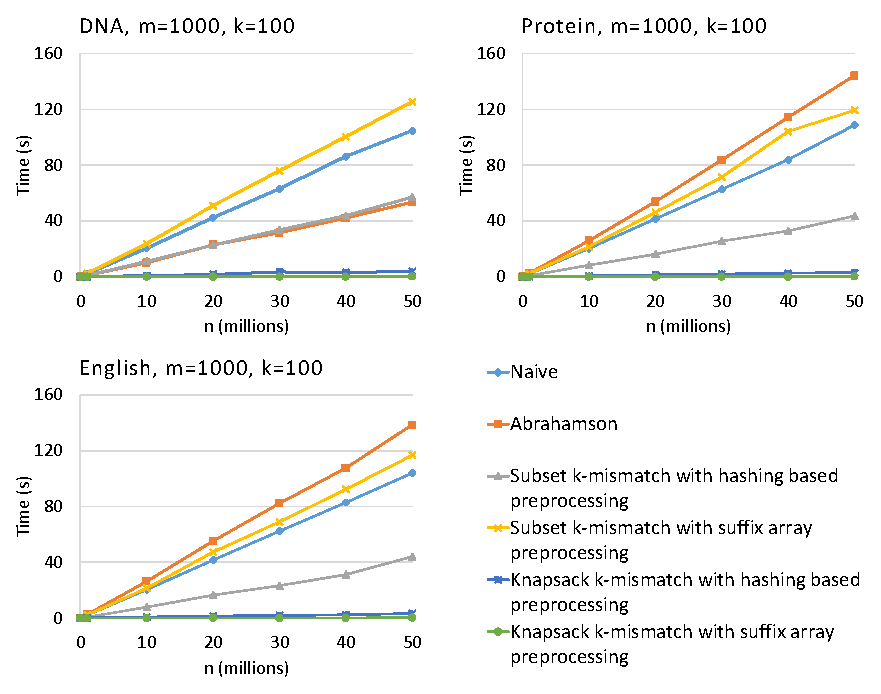
\includegraphics{fig1.eps}

Run times for pattern matching on DNA, protein and
English alphabet data, when the length of the text ($n$) varies.
The length of the pattern is $m=1000$. The maximum number of mismatches
allowed is $k=100$.
Our algorithms are Subset
k-mismatch with hashing based preprocessing (section
\ref{sec_k_mism_det}), Subset k-mismatch with suffix array preprocessing (section \ref{sec_k_mism_det}),
Knapsack k-mismatch with hashing based preprocessing (section
\ref{sec_nsqrtk}), and Knapsack k-mismatch with suffix array preprocessing (section
\ref{sec_nsqrtk}). 
\end{figure*}



\begin{figure*}
\caption{Run times for pattern matching when the length of the pattern
varies.}
\includegraphics{fig2.eps}

Run times for pattern matching on DNA, protein and
English alphabet data, when the length of the pattern ($m$) varies.
The length of the text is $n = 10$ millions. The maximum number of
mismatches allowed is $k=10\%$ of the pattern length.
Our algorithms are Subset
k-mismatch with hashing based preprocessing (section
\ref{sec_k_mism_det}), Subset k-mismatch with suffix array preprocessing (section \ref{sec_k_mism_det}),
Knapsack k-mismatch with hashing based preprocessing (section
\ref{sec_nsqrtk}), and Knapsack k-mismatch with suffix array preprocessing (section
\ref{sec_nsqrtk}).
\label{fig_runtimes_varym} 
\end{figure*}



\begin{figure*}
\caption{Run times for pattern matching when the maximum number of mismatches
allowed varies.}
\label{fig_runtimes_varyk} 
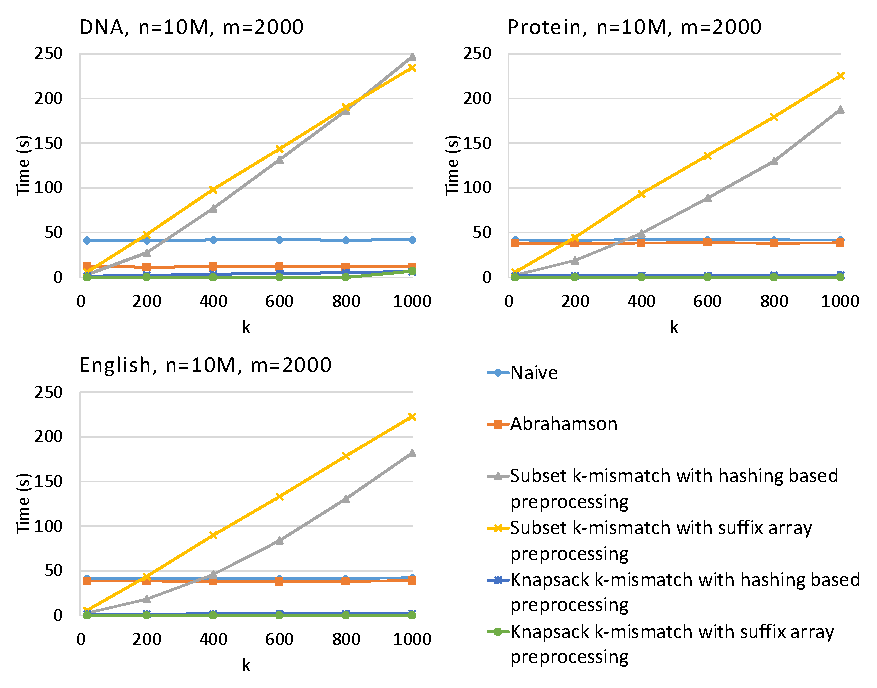
\includegraphics{fig3.eps} 

Run times for pattern matching on DNA, protein and
English alphabet data, when the maximum number of mismatches allowed ($k$)
varies.
The length of the text is $n=10$ millions. The length of the pattern is
$m=2000$.
Our algorithms are Subset
k-mismatch with hashing based preprocessing (section
\ref{sec_k_mism_det}), Subset k-mismatch with suffix array preprocessing (section \ref{sec_k_mism_det}),
Knapsack k-mismatch with hashing based preprocessing (section
\ref{sec_nsqrtk}), and Knapsack k-mismatch with suffix array preprocessing (section
\ref{sec_nsqrtk}). 
\end{figure*}



\begin{figure*}
\caption{Run times for pattern matching when the size of the alphabet varies.}
\label{fig_runtimes_varySigma} 
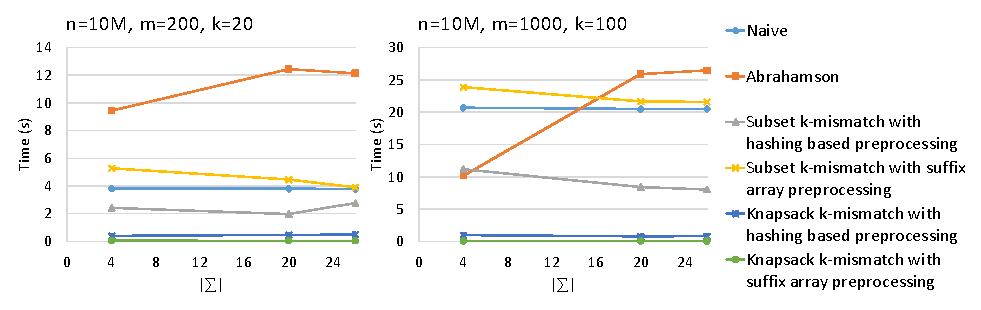
\includegraphics[width=\linewidth]{fig4.eps} 

Run times for pattern matching when the size of the alphabet varies
from 4 (DNA) to 20 (protein) to 26 (English).
The length of the text is $n=10$ millions. The length of the pattern is
$m=200$ in the first graph and $m=1000$ in the second. The maximum number of
mismatches allowed is $k=20$ in the first graph and $k=100$ in the second.
Our algorithms are Subset k-mismatch with hashing based
preprocessing (section \ref{sec_k_mism_det}), Subset k-mismatch with suffix array preprocessing (section \ref{sec_k_mism_det}),
Knapsack k-mismatch with hashing based preprocessing (section
\ref{sec_nsqrtk}), and Knapsack k-mismatch with suffix array preprocessing (section
\ref{sec_nsqrtk}). 
\end{figure*}


\section{Conclusions}
We have  introduced several deterministic and randomized, exact and
approximate algorithms for pattern matching with mismatches and the $k$-mismatches
problems, with or without wild cards. These algorithms improve the run time, 
simplify, or extend previous algorithms wild cards. 
We have also implemented some of the deterministic algorithms. An empirical
comparison of these algorithms showed that the algorithms based on
character comparison outperform those based on convolutions.